% Options for packages loaded elsewhere
\PassOptionsToPackage{unicode}{hyperref}
\PassOptionsToPackage{hyphens}{url}
%
\documentclass[
  11pt,
  twocolumn]{article}
\usepackage{amsmath,amssymb}
\usepackage{lmodern}
\usepackage{iftex}
\ifPDFTeX
  \usepackage[T1]{fontenc}
  \usepackage[utf8]{inputenc}
  \usepackage{textcomp} % provide euro and other symbols
\else % if luatex or xetex
  \usepackage{unicode-math}
  \defaultfontfeatures{Scale=MatchLowercase}
  \defaultfontfeatures[\rmfamily]{Ligatures=TeX,Scale=1}
\fi
% Use upquote if available, for straight quotes in verbatim environments
\IfFileExists{upquote.sty}{\usepackage{upquote}}{}
\IfFileExists{microtype.sty}{% use microtype if available
  \usepackage[]{microtype}
  \UseMicrotypeSet[protrusion]{basicmath} % disable protrusion for tt fonts
}{}
\makeatletter
\@ifundefined{KOMAClassName}{% if non-KOMA class
  \IfFileExists{parskip.sty}{%
    \usepackage{parskip}
  }{% else
    \setlength{\parindent}{0pt}
    \setlength{\parskip}{6pt plus 2pt minus 1pt}}
}{% if KOMA class
  \KOMAoptions{parskip=half}}
\makeatother
\usepackage{xcolor}
\usepackage[margin=0.5in]{geometry}
\usepackage{graphicx}
\makeatletter
\def\maxwidth{\ifdim\Gin@nat@width>\linewidth\linewidth\else\Gin@nat@width\fi}
\def\maxheight{\ifdim\Gin@nat@height>\textheight\textheight\else\Gin@nat@height\fi}
\makeatother
% Scale images if necessary, so that they will not overflow the page
% margins by default, and it is still possible to overwrite the defaults
% using explicit options in \includegraphics[width, height, ...]{}
\setkeys{Gin}{width=\maxwidth,height=\maxheight,keepaspectratio}
% Set default figure placement to htbp
\makeatletter
\def\fps@figure{htbp}
\makeatother
\setlength{\emergencystretch}{3em} % prevent overfull lines
\providecommand{\tightlist}{%
  \setlength{\itemsep}{0pt}\setlength{\parskip}{0pt}}
\setcounter{secnumdepth}{-\maxdimen} % remove section numbering
\newlength{\cslhangindent}
\setlength{\cslhangindent}{1.5em}
\newlength{\csllabelwidth}
\setlength{\csllabelwidth}{3em}
\newlength{\cslentryspacingunit} % times entry-spacing
\setlength{\cslentryspacingunit}{\parskip}
\newenvironment{CSLReferences}[2] % #1 hanging-ident, #2 entry spacing
 {% don't indent paragraphs
  \setlength{\parindent}{0pt}
  % turn on hanging indent if param 1 is 1
  \ifodd #1
  \let\oldpar\par
  \def\par{\hangindent=\cslhangindent\oldpar}
  \fi
  % set entry spacing
  \setlength{\parskip}{#2\cslentryspacingunit}
 }%
 {}
\usepackage{calc}
\newcommand{\CSLBlock}[1]{#1\hfill\break}
\newcommand{\CSLLeftMargin}[1]{\parbox[t]{\csllabelwidth}{#1}}
\newcommand{\CSLRightInline}[1]{\parbox[t]{\linewidth - \csllabelwidth}{#1}\break}
\newcommand{\CSLIndent}[1]{\hspace{\cslhangindent}#1}
\usepackage{hyperref}
\usepackage{array}
\usepackage{caption}
\usepackage{graphicx}
\usepackage{multirow}
\usepackage{hhline}
\usepackage{calc}
\usepackage{tabularx}
\usepackage[para,online,flushleft]{threeparttable}
\DeclareMathOperator{\logit}{logit}
\DeclareMathOperator{\var}{var}
\usepackage{float}
\usepackage{booktabs}
\usepackage{longtable}
\usepackage{array}
\usepackage{multirow}
\usepackage{wrapfig}
\usepackage{colortbl}
\usepackage{pdflscape}
\usepackage{tabu}
\usepackage{threeparttable}
\usepackage{threeparttablex}
\usepackage[normalem]{ulem}
\usepackage{makecell}
\usepackage{xcolor}
\ifLuaTeX
  \usepackage{selnolig}  % disable illegal ligatures
\fi
\IfFileExists{bookmark.sty}{\usepackage{bookmark}}{\usepackage{hyperref}}
\IfFileExists{xurl.sty}{\usepackage{xurl}}{} % add URL line breaks if available
\urlstyle{same} % disable monospaced font for URLs
\hypersetup{
  pdftitle={Analysis of Health Survey for England (HSE) 2019},
  pdfauthor={Candidate Numbers Here},
  hidelinks,
  pdfcreator={LaTeX via pandoc}}

\title{Analysis of Health Survey for England (HSE) 2019}
\author{Candidate Numbers Here}
\date{March 13, 2024}

\begin{document}
\maketitle
\begin{abstract}
This report provides an analysis of data related to health, age,
socio-economic factors and lifestyle habits in adults (from the age of
16) from the population in England, derived from the Health Survey for
England 2019.
\end{abstract}

\pagenumbering{gobble}

\clearpage

\hypertarget{summary}{%
\section{Summary}\label{summary}}

In England, smoking, ``vaping'' and alcohol consumption are widespread
habits among adults, particularly younger adults. In fact, it is
estimated that around 13.9\% of adults in England identified as
cigarette smokers (\protect\hyperlink{ref-1ONS}{ONS 2019a}), and a
similar study found that there were 10.9 alcohol-related deaths per
100,000 people living in England in 2019
(\protect\hyperlink{ref-2ONS}{ONS 2019b}). Thus, it is crucial to be
aware of the predictors and consequences of these habits, which is the
motivation for this analysis.

We conducted this analysis on a subset containing 8,204 adults living in
England (ages 16+), who were interviewed in their homes about their
demographics and their smoking and drinking habits as part of the Health
Survey for England (HSE) 2019. 4,947 of these participants who consented
to an at-home nurse visit had vitals such as blood pressure, weight and
height measured. We investigated which features of a participant are
associated with smoking habits, and which habits are associated with
high blood pressure.

\textbf{This is where our non-technical summary of results should go}

\hypertarget{introduction}{%
\subsection{Introduction}\label{introduction}}

The mechanisms which drive lifestyle habits are part of a complex and
ever-changing field in behavioural psychology. What is known, however,
is that such habits are driven by cues and cravings {[}Anastasia
Droungas
(\protect\hyperlink{ref-SmokeCue}{1995}){]}(\protect\hyperlink{ref-DrinkCue}{Kambouropoulos
2009}). The HSE 2019 captures demographic and socioeconomic
characteristics that have the potential to make such cues more visible
and cravings harder to resist. For example, living in a region where
smoking is more prevalent or not having a husband/wife for an
accountability partner to help you quit or resist these habits
(\protect\hyperlink{ref-AccountPartner}{ONS 2019c}).

In this report, we will use weighting variables to estimate prevalence
of cigarette, e-cig, and alcohol users in our population, and compare it
with the larger population of adults in England. We will then attempt to
identify associations with a participants current smoking status,
explore whether predictive modelling can be used to identify smokers
with a high accuracy, and investigate which lifestyle habits are
associated with increased values of systolic blood pressure. \emph{This
will be crucial in enabling healthcare providers to implement
preventative care for people at risk of developing hypertension.}

\hypertarget{methodology}{%
\section{Methodology}\label{methodology}}

\hypertarget{exploratory-analysis}{%
\subsection{Exploratory Analysis}\label{exploratory-analysis}}

The full HSE 2019 cross-sectional data set contains 10,299 observations
across thousands of variables (\protect\hyperlink{ref-Main}{NatCen
Social Research and Health 2019}), but we only studied patients over the
age of 16 among key variables. Our subset includes 8,204 participants
and 19 variables, which are described in Table
\ref{tab:output-var-table}.

\begin{table}
\centering
\caption{\label{tab:outputvartable}Summary of the analysis variables used in our report. (D) indicates that a variable was derived.\label{tab:output-var-table}}
\centering
\fontsize{10}{12}\selectfont
\begin{tabular}[t]{>{\raggedright\arraybackslash}p{6em}|>{\raggedright\arraybackslash}p{10em}|l}
\hline
\textbf{Variable} & \textbf{Definition} & \textbf{Notation}\\
\hline
SerialA & Respondent serial number & NA\\
\hline
wt\_int & Weight of observation & NA\\
\hline
Sex & Respondent sex (M/F) & $s$\\
\hline
(D) Age35g & Respondent age grouped in 5 year bands for 16+ & $a^{(5)}$\\
\hline
(D) ag16g10 & Respondent age grouped in 10 year bands for 16+ & $a^{(10)}$\\
\hline
(D) topqual2 & Highest level qualification & $t$\\
\hline
(D) marstatD & Marital status & $m$\\
\hline
(D) qimd19 & IMD score (a measure of deprivation) & $q$\\
\hline
(D) urban14b & Level of rurality & $u$\\
\hline
(D) origin2 & Grouped ethnic category & $o$\\
\hline
(D) cigdyal\_19 & $\#$ of cigarettes smoked per day & $n^{cig}$\\
\hline
(D) cigsta3\_19 & Smoking status (Reg / Ex-Reg / Never-Reg) & $cig$\\
\hline
(D) NDPNow\_19 & Use of E-cigarettes and or NDPs & $ndp$\\
\hline
(D) DrinkYN\_19 & Alcohol consumed in the last 12 months & $alc$\\
\hline
dnoft\_19 & Frequency of alcohol consumed in the last 12 months (grouped) & NA\\
\hline
(D) d7many3\_19 & $\#$ of days alcohol was consumed in the last week & $n^{alc}$\\
\hline
(D) GOR1 & Government region office number & $g$\\
\hline
(D) BMIval & Valid BMI measurement (weight estimated if $\>$ 130kg) & $bmi$\\
\hline
(D) omsysval & Valid mean systolic blood pressure & $sbp$\\
\hline
\end{tabular}
\end{table}

\hypertarget{duplicates}{%
\subsubsection{Duplicates}\label{duplicates}}

We found 36 pairs of observations with exactly equal variables
(excluding ID variables and lab measurements), but we did not remove
these from our analysis because the supporting documentation didn't
state a protocol for repeated visits. We assumed these were genuine
observations from different participants and thus included them in our
dataset. However, there were 3 pairs of observations that had duplicate
lab variables also. We believed that these were true duplicates and
removed one observation from each of the three pairs resulting in a
dataset of 8201 observations.

\hypertarget{dichotomy-of-factors}{%
\subsubsection{Dichotomy of Factors}\label{dichotomy-of-factors}}

All variables were originally coded as numeric in our dataset, so we
recoded these to factor variables accordingly. Some of the variables
used for analysis were dichotomised by us for easier interpretation. We
coded a binary variable indicating current smoking status, which will
serve as our \emph{primary} outcome variable. Also, we dichotomised
urbanity into two levels being `Rural' and `Urban', and finally marital
status into `Married' and `Not Married'. We group respondents into
`Higher Education', `Further Education', `A-Level equiv.', `GCSE
equiv.', `No qualification' and `Foreign/other'.

\hypertarget{missingness}{%
\subsubsection{Missingness}\label{missingness}}

The number of missing observations for each are shown in Table
\ref{tab:output-na-table}:

\begin{table}
\centering
\caption{\label{tab:outputnatable}Missing values in the training dataset\label{tab:output-na-table}}
\centering
\fontsize{9}{11}\selectfont
\begin{tabular}[t]{l|r|l}
\hline
\textbf{Variable} & \textbf{Missing Values} & \textbf{\% Missing}\\
\hline
omsysval & 4036 & 61.5\%\\
\hline
BMIVal & 1519 & 23.2\%\\
\hline
dnoft\_19 & 1496 & 22.8\%\\
\hline
cigdyal\_19 & 57 & 0.869\%\\
\hline
cigsta3\_19 & 56 & 0.854\%\\
\hline
NDPNow\_19 & 53 & 0.808\%\\
\hline
d7many3\_19 & 52 & 0.793\%\\
\hline
drinkYN\_19 & 51 & 0.777\%\\
\hline
topqual2 & 46 & 0.701\%\\
\hline
origin2 & 29 & 0.442\%\\
\hline
marstatD & 1 & 0.0152\%\\
\hline
\end{tabular}
\end{table}

There is significant missingness in the lab values, which can be
explained by the fact additional consent was needed from the participant
to allow a nurse visit. One variable with a substantial amount of data
missing was the frequency of drinking in the last 12 months, which due
to the retrospective and sensitive nature of the question could be
explained by either recall bias or a participant's refusal to answer. As
a result, we decided to remove this variable from analysis in favour of
a binary variable which simply states whether the respondent has drunk
alcohol in the last 12 months. Education level, marital status and
ethnicity are the only socioeconomic variables with any missing entries,
with 46 observations (0.701\% of the data) missing at least one of the
three. These are not necessary for identifiability and as they are
sensitive, we do not expect every participant to answer these questions.
Therefore, we did not remove these observations.

\hypertarget{outliers-and-data-issues}{%
\subsubsection{Outliers and Data
Issues}\label{outliers-and-data-issues}}

We attempted to determine whether the two lab measurement variables
contained potential outliers, and as can be seen in Figure
@ref(tab:output distribution plots), there were many outliers for BMI.
We note that this used self-estimated weight from the participant in the
calculation when it exceeded 130kg. Additionally, weight measurements
were taken in inconsistent environments such as on different flooring in
the participants' homes which will impact measurement accuracy. We
believed this could have explained the extremely high BMI values in the
range of 54.82 to 73.49. We coded such values as missing in the analysis
dataset, but kept the observation.

The readings for systolic blood pressure were collected by taking an
average of three readings, each five minutes apart, performed by a
trained nurse who had to declare each reading to be valid. For this
reason, it seemed highly unlikely that these readings were mistakes, and
so we included them in our analysis. The measurement device used has
been validated for use in this environment
(\protect\hyperlink{ref-Omron}{Yechiam Ostchega PhD 2009}). We did,
however, note that values of systolic blood pressure that were this
consistently high (\textgreater140mmHg) were indicators for hypertensive
crisis, and so a part of our population may have serious underlying
health conditions that could affect the generalisability of our findings
(\protect\hyperlink{ref-heart}{Association 2023}).

\begin{figure}[H]
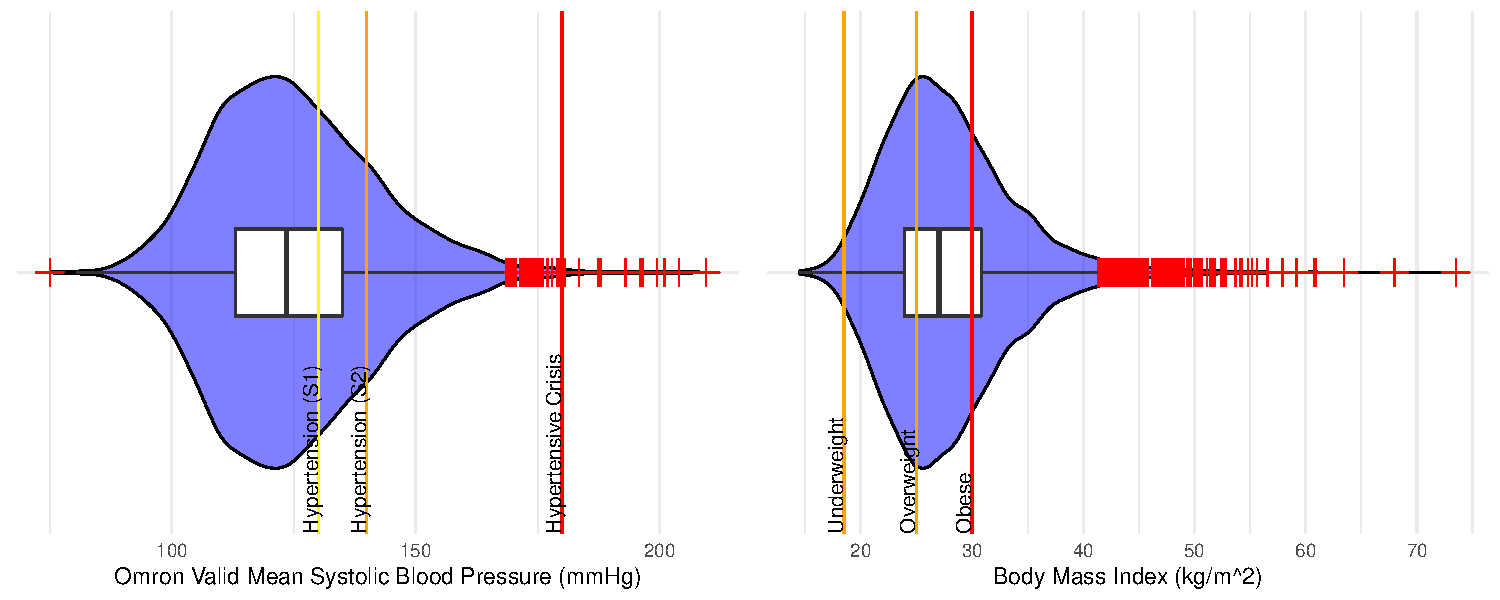
\includegraphics{Coursework_files/figure-latex/output-distribution-plots-1} \caption{Distribution of BMI and Mean Systolic Blood Pressure}\label{fig:output-distribution-plots}
\end{figure}

\hypertarget{analysis}{%
\subsection{Analysis}\label{analysis}}

\hypertarget{what-is-the-prevelence-of-drinking-smoking-and-e-cig-usage}{%
\subsubsection{What is the prevelence of drinking, smoking and E-cig
usage?}\label{what-is-the-prevelence-of-drinking-smoking-and-e-cig-usage}}

To calculate the prevalence of these three habits we assumed each of the
\(n\) observations, \(x_1,…,x_n\) , to be independent, identically
distributed (iid) random variables (RVs) where
\(x_i \sim Bern(p)\, \forall i=1,…,n\) and \(p\) denotes the probability
of a habit being present for the given observation.

We used the household-level weighting variable to calculate a weighted
Maximum Likelihood Estimate (MLE) of \(p\). That is, letting \(w_i\)
denote the weight of the \(i^{th}\) observation, we altered the standard
likelihood function of a Bernoulli distribution as below:

\[L(p|\textbf{x}) = \prod_{i = 1}^{n} (p^{x_i}(1-p)^{1-x_i})^{w_i}\]
From this, we calculated our weighted MLE as
\(\widehat{p} = \frac{\sum_{i=1}^{n} x_iw_i}{\sum_{i=1}^{n} w_i}\). It
can also be shown that the MLE has variance given by
\(\mathop{\mathrm{var}}(\widehat{p})=\frac{p(1-p)}{\sum_{i=1}^{n}w_i}\),
which we estimated using \(\widehat{p}\). We used large sample
properties of the MLE to get a normal approximation and estimated 95\%
confidence intervals for each habit, which are shown in Table
\ref{tab:output-estimates-table}.

\begin{table}
\centering
\caption{\label{tab:outputestimatestable}Estimates and 95\% Confidence Intervals for \% of Population\label{tab:output-estimates-table}}
\centering
\fontsize{9}{11}\selectfont
\begin{tabular}[t]{l|l|l}
\hline
\textbf{Habit} & \textbf{Estimate} & \textbf{C.I.}\\
\hline
Drinking & 80.4\% & (79.5\%, 81.2\%)\\
\hline
Smoking & 16.5\% & (15.7\%, 17.3\%)\\
\hline
Smoking E-cigarettes & 4.28\% & (3.84\%, 4.72\%)\\
\hline
\end{tabular}
\end{table}

We found that the usage of e-cigarette usage among adults is relatively
low, making it challenging to dissect any significant trends within the
data. \emph{Maybe a wee bit more here}

\hypertarget{how-is-smoking-associated-with-socioeconomic-factors-and-age}{%
\subsubsection{How is smoking associated with socioeconomic factors and
age?}\label{how-is-smoking-associated-with-socioeconomic-factors-and-age}}

Next, we worked to uncover factors that have possible associations with
smoking prevalence. We started with the demographic factors of age and
gender, plotting the smoking prevalence across combinations of these
groups to identify any patterns. Figure \ref{fig:output-prevelance-plot}
suggests a negative correlation between age and the proportion of
current cigarette smokers, across both genders. Interestingly, the
proportion of males who quit smoking in later-life was much greater than
that of females (75yrs+; M: 50\%, F: 31\%).

\begin{figure}[H]
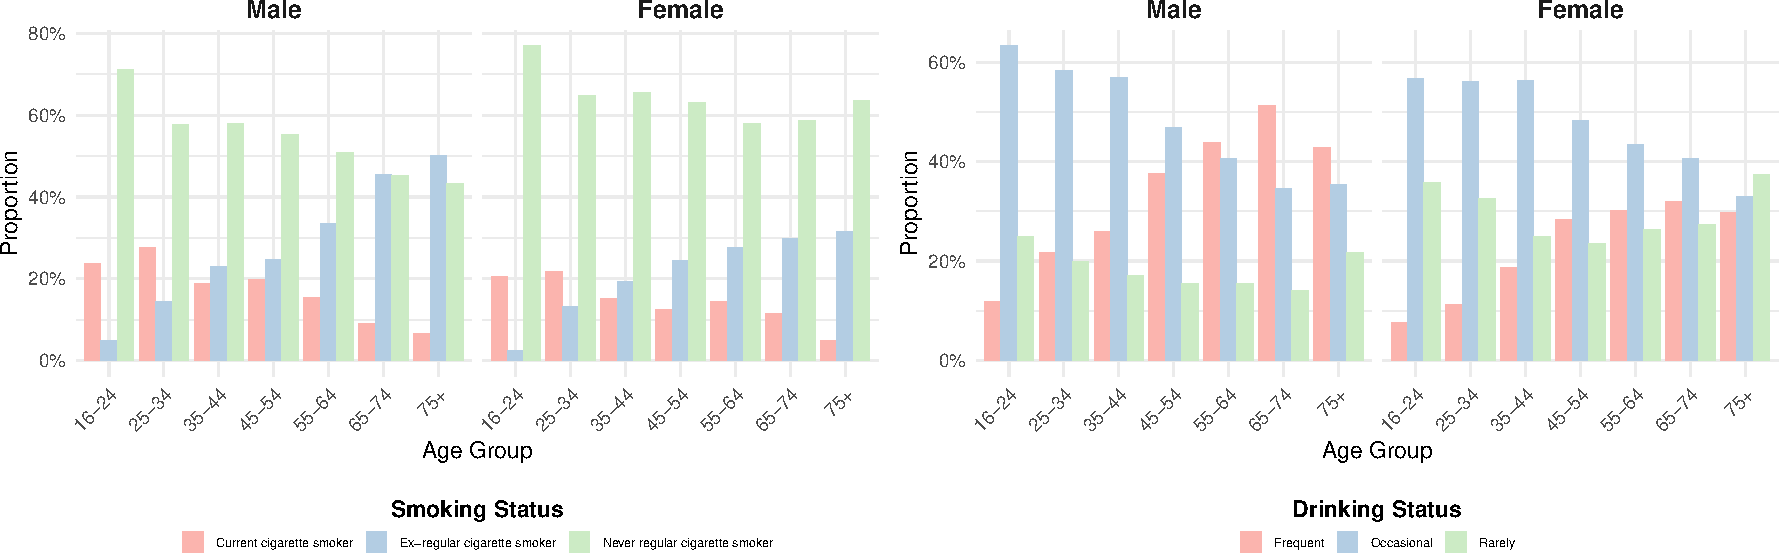
\includegraphics{Coursework_files/figure-latex/output-smoking-drinking-age-plot-1} \caption{Smoking and drinking status proportions by age group and gender}\label{fig:output-smoking-drinking-age-plot}
\end{figure}

\begin{figure}[H]
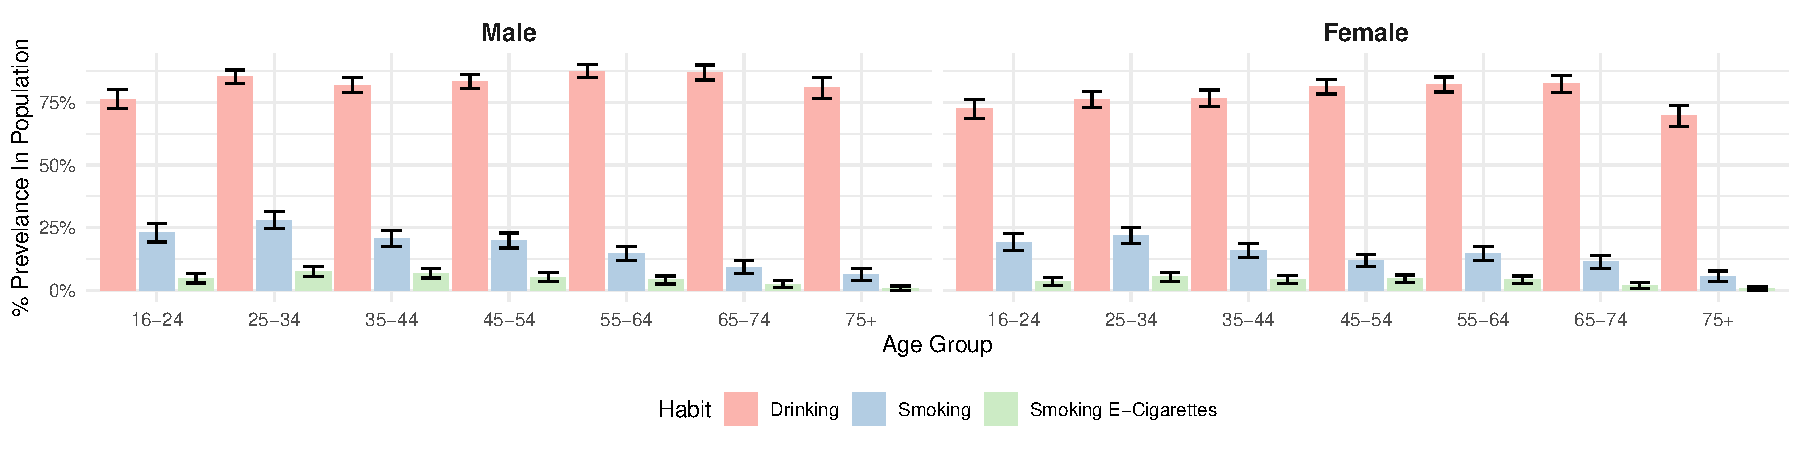
\includegraphics{Coursework_files/figure-latex/output-prevelance-plot-1} \caption{Estimation of the prevelance of smokers by deprivation}\label{fig:output-prevelance-plot}
\end{figure}

\emph{Additionally, males demonstrate a higher prevalence of drinking
across nearly all demographic categories in comparison to females.}
\emph{We can clearly see that smoking prevalence increases with our
deprivation variable, meaning that smokers tend to be from lower levels
of deprivation. This correlation may be caused by the hefty tobacco
duties the UK impose on its' residents
(\protect\hyperlink{ref-GovUK}{GOV.UK 2014}). Less deprived individuals
they can take-up more unnecessary, expensive habits, with smoking being
one of the main candidates.}

We reserved 80\% of our data to train the model, and used the remaining
20\% to test the model, which was made possible due to the large size of
our dataset. The training set contained 6561 observations and the test
set contained 1640. \emph{Table \ref{tab:output-testtrain-table}
summarises the key variables between the test and train dataset to
illustrate that both are representative of the whole dataset.} This
reduced the risk of overfitting and allowed us to test the predictive
power of each model we proposed.

\begin{table}
\centering
\caption{\label{tab:outputtesttraintable}Comparison of the characteristics of the training set compared with the test set.\label{tab:output-testtrain-table}}
\centering
\fontsize{10}{12}\selectfont
\begin{tabular}[t]{l|l|l}
\hline
\multicolumn{1}{c|}{ } & \multicolumn{2}{c}{Proportion (\%)} \\
\cline{2-3}
\textbf{Variable:Label} & \textbf{Test} & \textbf{Train}\\
\hline
Sex:Male & 46.6 & 44.8\\
\hline
Sex:Female & 53.4 & 55.2\\
\hline
 &  \vphantom{3} & \\
\hline
topqual2:No qualification & 17.4 & 18.0\\
\hline
topqual2:GCSE equiv. & 20.7 & 21.2\\
\hline
topqual2:A-Level equiv. & 13.5 & 13.8\\
\hline
topqual2:Further Education & 29.7 & 29.3\\
\hline
topqual2:Higher Education & 17.6 & 16.4\\
\hline
topqual2:Foreign/Other & 1.1 & 1.1\\
\hline
 &  \vphantom{2} & \\
\hline
marstatD:Married & 54.5 & 52.5\\
\hline
marstatD:Not Married & 45.5 & 47.5\\
\hline
 &  \vphantom{1} & \\
\hline
urban14b:Urban & 82.2 & 81.0\\
\hline
urban14b:Not Urban & 17.8 & 19.0\\
\hline
 &  & \\
\hline
origin2:White & 85.0 & 86.0\\
\hline
origin2:Black & 2.6 & 2.8\\
\hline
origin2:Asian & 10.1 & 8.5\\
\hline
origin2:Multiple & 1.9 & 1.6\\
\hline
origin2:Other & 0.5 & 1.0\\
\hline
\textbf{} & \textbf{Mean} & \textbf{Mean}\\
\hline
Age(Estimated) &  & \\
\hline
\end{tabular}
\end{table}

To develop a predictive model for identifying smokers, we used the
binary variable for current smoking status as a response, with various
socioeconomic and demographic factors as predictors. These were selected
based on the associations suggested by our prior analysis.

Under the assumption that the age of participants were approximately
uniformly distributed within their respective age bands, we defined the
estimated age of the \(i^{th}\) observation as the midpoint of the
participants respective 5-year age group (taking the estimation of the
90+ category as 92.5), denoted \(a_i\). We found that age may represent
a somewhat quadratic effect on the probability of smoking, leading us to
include a \(a_i^2\) term in our model. A comparison of these models are
summarised in Table \ref{tab:output-model-selection-table}.

\begin{table}
\centering
\caption{\label{tab:outputmodelselectiontable}Comparison of selected model evaluations, wherein $\eta_i = \text{logit}(\mu_i)$, and Acc. refers to the model accuracy on test data.\label{tab:output-model-selection-table}}
\centering
\fontsize{9}{11}\selectfont
\begin{tabular}[t]{>{\raggedright\arraybackslash}p{7em}|r|r|r|r|r}
\hline
\multicolumn{3}{c|}{ } & \multicolumn{2}{c|}{RMSE} & \multicolumn{1}{c}{ } \\
\cline{4-5}
\textbf{Model} & \textbf{AIC} & \textbf{AUC} & \textbf{Train} & \textbf{Test} & \textbf{Acc.}\\
\hline
$\eta_i \sim a_i + a_i^2 + ms_i + q_i + u_i + o_i + t_i + s_i + q_i:u_i$ & 4987.5 & 0.759 & 0.342 & 0.324 & 0.861\\
\hline
$\eta_i \sim a_i + a_i^2 + ms_i + q_i + u_i + o_i + t_i + s_i$ & 4987.3 & 0.759 & 0.342 & 0.324 & 0.861\\
\hline
$\eta_i \sim a_i + ms_i + q_i + u_i + o_i + t_i + s_i$ & 5036.4 & 0.740 & 0.343 & 0.327 & 0.861\\
\hline
$\eta_i \sim a_i^{(5)} + ms_i + q_i + u_i + o_i + t_i + s_i$ & 4994.3 & 0.759 & 0.341 & 0.325 & 0.861\\
\hline
$\eta_i \sim a_i^{(10)} + ms_i + q_i + u_i + o_i + t_i + s_i$ & 5005.9 & 0.753 & 0.342 & 0.324 & 0.860\\
\hline
\end{tabular}
\end{table}

We selected the model based on AIC, which enabled us to balance model
complexity and model fit (quantified by likelihood), which further
reduced the risk of overfitting. This model is \emph{change factors}

\[\text{logit}(\mu_i) \sim \beta_0 + \beta_1a + \beta_2a^2 + \beta_3q + \alpha^{ms}_j + \alpha^{u}_k + \alpha^{o}_l + \alpha^{t}_m + \alpha^{s}_n\]
where \(j \in \{\text{Married, Not Married}\}\),
\(k \in \{\text{Urban, Not Urban}\}\),
\(l \in \{\text{White, Asian, Black, Multiple, Other}\}\),
\(n \in \{\text{Male, Female}\}\) and
\(m \in \{\text{Higher Education, A-Level equiv., Further Education, GCSE equiv., Foreign/Other, No qualification}\}\).

To evaluate the predictive performance of our final model using our test
data, Figure 4 demonstrates the predicted probability of each
`probability bin' against the mean actual outcomes. As we can see the
calibration curve closely follows the line \(y = x\), which is
indicative of a well-calibrated model.

\emph{This model doesn't predict high values\ldots{} answer why}

\begin{figure}[H]

{\centering 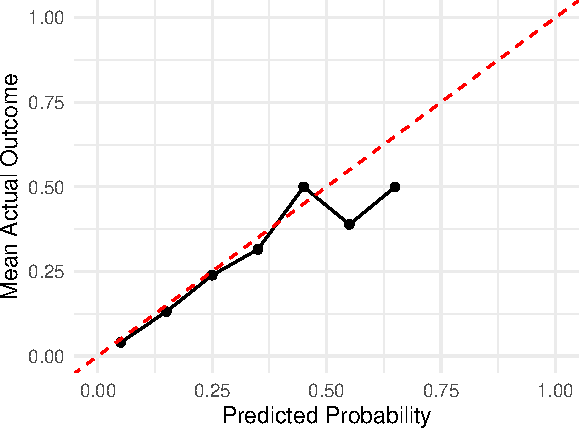
\includegraphics{Coursework_files/figure-latex/output-calibration-chart-1} 

}

\caption{Calibration chart for Binomial model}\label{fig:output-calibration-chart}
\end{figure}

\hypertarget{which-lifestyle-habits-are-associated-with-systolic-blood-pressure}{%
\subsubsection{Which lifestyle habits are associated with systolic blood
pressure?}\label{which-lifestyle-habits-are-associated-with-systolic-blood-pressure}}

For this analysis, we filtered out any observations that had any lab
values missing.

\begin{figure}[H]
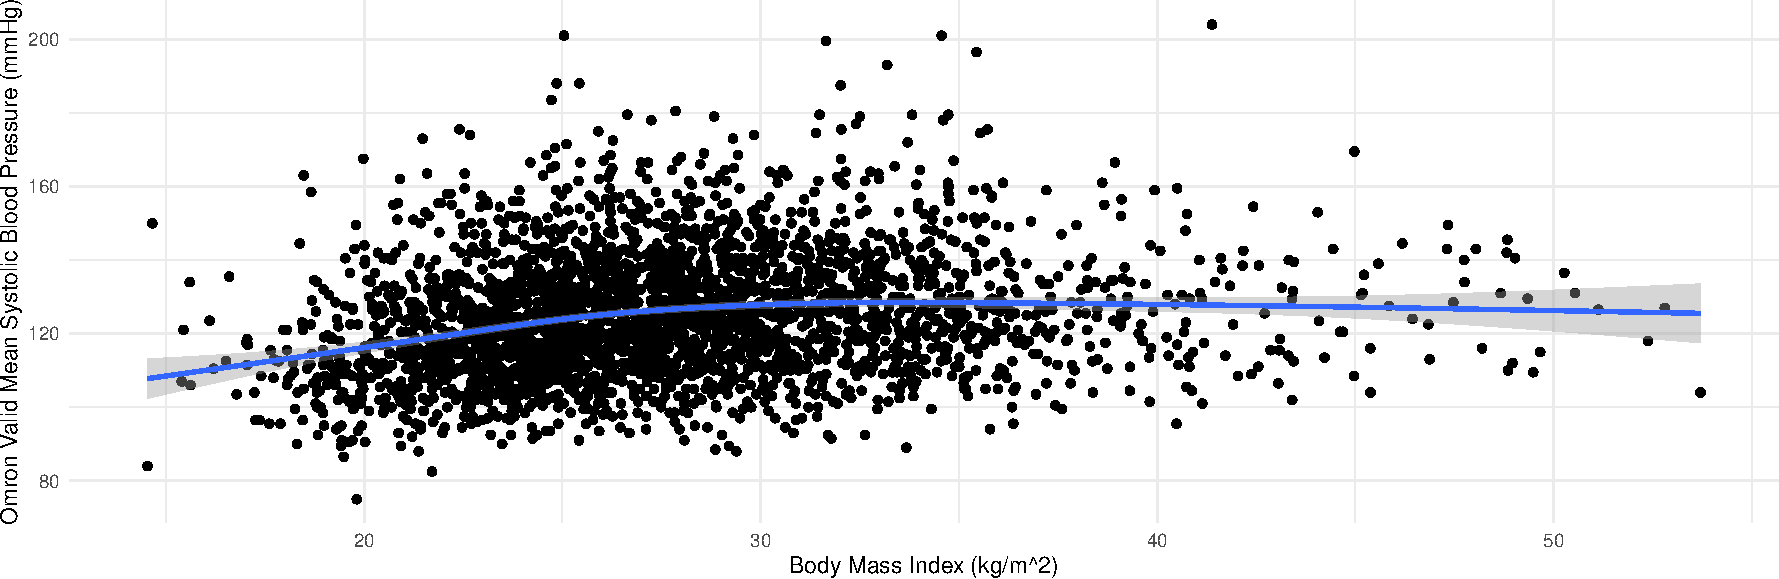
\includegraphics{Coursework_files/figure-latex/output relationship plots-1} \caption{Relationship of BMI and Age with Mean Systolic Blood Pressure}\label{fig:output relationship plots}
\end{figure}

\begin{figure}[H]

{\centering 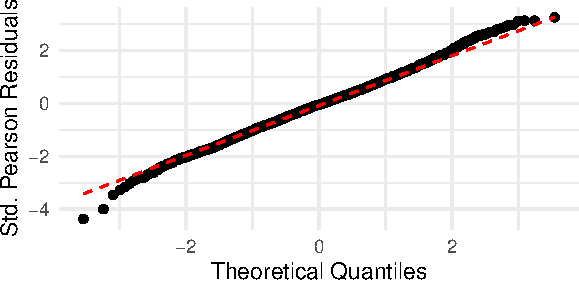
\includegraphics{Coursework_files/figure-latex/output qq plot for q3-1} 

}

\caption{Q-Q plot of Inverse-Normal model residuals}\label{fig:output qq plot for q3}
\end{figure}

\hypertarget{resultsconclusion}{%
\subsection{Results/Conclusion}\label{resultsconclusion}}

Our analysis showed that alcohol consumption is extremely common among
UK adults, with approximately 80.4\% being consumers, while smoking and
vaping rates are lower at 16.5\% and 4.3\%, respectively. Older males
show the highest tendencies for alcohol consumption, with `frequent'
drinking the most prevalent among males aged 65-74. Unlike `frequent'
alcohol consumption, the prevalence of smoking decreases with age.
Individuals aged 16-24 appear to be the worst offenders when it comes to
smoking cigarettes, indicating a significant issue within youth culture.
Moreover, we found an interesting relationship between deprivation
levels and smoking and drinking behaviours. Smoking prevalence seemed to
increase as deprivation levels decrease, while alcohol consumption
appeared to do the opposite.

To help us uncover the underlying socio-economic factors that may drive
the prevalence of smoking, we first looked at the most `comparable'
respondent type in our dataset. This `respondent' is a white, single
male who has no qualifications and lives in an urban area. We found that
the probability of our hypothetical respondent being a smoker is
approximately 25\% \emph{Where is this from?} (notably higher than the
population average of 16.5). \emph{Maybe worth talking about confidence
intervals here - is value outside 95\%} The only socio-economic
variables to certainly increase this probability is the deprivation
level our respondent falls under. The rest of the socio-economic
variables we have access to, appear to decrease the likelihood of
smoking. For example, if our respondent is any of the following: Asian,
black, married, or went on to further education, the chances of them
being a smoker is at-least halved.

\clearpage

\hypertarget{references}{%
\section*{References}\label{references}}
\addcontentsline{toc}{section}{References}

\hypertarget{refs}{}
\begin{CSLReferences}{1}{0}
\leavevmode\vadjust pre{\hypertarget{ref-SmokeCue}{}}%
Anastasia Droungas, Anna Rose Childress, Ronald N. Ehrman. 1995.
{``{Effect of smoking cues and cigarette availability on craving and
smoking behavior}.''}
\url{https://www.sciencedirect.com/science/article/pii/030646039500029C}.

\leavevmode\vadjust pre{\hypertarget{ref-heart}{}}%
Association, American Heart. 2023. {``{Understanding Blood Pressure
Readings}.''}
\url{https://www.heart.org/en/health-topics/high-blood-pressure/understanding-blood-pressure-readings}.

\leavevmode\vadjust pre{\hypertarget{ref-GovUK}{}}%
GOV.UK. 2014. {``{Tax on shopping and services}.''}
\url{https://www.gov.uk/tax-on-shopping/alcohol-tobacco}.

\leavevmode\vadjust pre{\hypertarget{ref-DrinkCue}{}}%
Kambouropoulos, Nicolas. 2009. {``{{`Cue reward salience'} predicts
craving in response to alcohol cues}.''}
\url{https://www.sciencedirect.com/science/article/abs/pii/S0191886908003127}.

\leavevmode\vadjust pre{\hypertarget{ref-Main}{}}%
NatCen Social Research, Department of Epidemiology, University College
London, and Public Health. 2019. {``{Health Survey for England}.''}
\url{http://doi.org/10.5255/UKDA-SN-8860-1}.

\leavevmode\vadjust pre{\hypertarget{ref-1ONS}{}}%
ONS. 2019a. {``{Adult smoking habits in the UK: 2019}.''}
\url{https://shorturl.at/qQW27}.

\leavevmode\vadjust pre{\hypertarget{ref-2ONS}{}}%
---------. 2019b. {``{Adult smoking habits in the UK: 2019}.''}
\url{https://shorturl.at/ftvwM}.

\leavevmode\vadjust pre{\hypertarget{ref-AccountPartner}{}}%
---------. 2019c. {``{Adult smoking habits in the UK: 2019}.''}
\url{https://shorturl.at/itPQU}.

\leavevmode\vadjust pre{\hypertarget{ref-Omron}{}}%
Yechiam Ostchega PhD, Tatiana Nwankwo MS, RN. 2009. {``{Assessing the
Validity of the Omron HEM-907XL Oscillometric Blood Pressure Measurement
Device in a National Survey Environment}.''}
\url{https://onlinelibrary.wiley.com/doi/full/10.1111/j.1751-7176.2009.00199.x}.

\end{CSLReferences}

\end{document}
